\documentclass[12pt]{paper}

\oddsidemargin 0.27in
\textwidth 5.9in
%\topmargin -.5in
\textheight 8.7in
\parindent 0em
\parskip 2ex

%\renewcommand{\baselinestretch}{1.5}

% New for newcommand, proglang and code
\newcommand{\pkg}[1]{{\normalfont\fontseries{b}\selectfont #1}}
\let\proglang=\textsf
\let\code=\texttt

\usepackage[utf8]{inputenc}
\usepackage[spanish]{babel}
\usepackage{verbatim} %poner comentarios largos
\usepackage[hang,small,sf]{caption}
\markright{}
\usepackage{graphicx}
\usepackage{amsfonts}
\usepackage{multicol}
\usepackage{hyperref}
\usepackage{amsmath,amsfonts,amsthm,amssymb,mathrsfs,latexsym}
\usepackage{textcomp}
\usepackage{multirow, array}
\usepackage[natbibapa]{apacite}
\usepackage{float}
\usepackage{comment}
\usepackage{mathrsfs}
\usepackage{upgreek}
\usepackage{makecell}

\usepackage{tikz}
\usetikzlibrary{arrows.meta, positioning, shapes.geometric}

\usepackage[numbib]{tocbibind}
\usepackage{xcolor}

\usepackage{adjustbox, array, hhline}
\renewcommand\theadfont{\normalfont\bfseries}
\renewcommand{\baselinestretch}{1.15}

%---------------------------------------------------------------------------------
\begin{document}
\renewcommand{\BOthers}[1]{et al.\hbox{}}

%---------------------------------------------------------------------------------
\newpage{\pagestyle{empty}\cleardoublepage}

\newpage
\begin{center}
\thispagestyle{empty} \vspace*{0cm} \textbf{\huge Proyecto de}\\ \textbf{\huge Maestría en Ciencias-Estadística} \\ [2.0cm]
\Large\textbf{Andrés Molina Escobar} \\
Estudiante de Maestría en Ciencias-Estadística\\[1.0cm]

\textbf{Comparación de metodologías estadísticas y de aprendizaje profundo para el modelamiento de la volatilidad en series financieras intradía.}\\[1.0cm]
Director:\\
Cesar Augusto Gomez Velez \\
Profesor Asistente,
Departamento de Estadística\\[1.0cm]

\centering

\includegraphics[scale=0.30]{las_figuras/logo_unal.png}

Universidad Nacional de Colombia \\
Departamento de Estadística \\
Medellín, Colombia \\
2026\\
\end{center}

\newpage
\tableofcontents
\newpage

\newpage

\section*{Resumen}
\addcontentsline{toc}{section}{Resumen}

Este trabajo evaluó y comparó el desempeño de tres metodologías para el pronóstico de la volatilidad en series financieras intradía: el modelo GARCH como representante de los enfoques estadísticos clásicos, y los modelos CEEMDAN-LSTM y PSOQRNN como representantes de los enfoques de aprendizaje profundo e híbridos. El estudio se realizó sobre seis activos financieros de distintas clases ---Bitcoin (BTC-USD), Ethereum (ETH-USD), oro (GC=F), el par de divisas EUR/USD, y los índices bursátiles S\&P\,500 y NASDAQ--- con datos intradía a 15 minutos acumulados entre febrero y julio de 2026. Los resultados muestran que el PSOQRNN supera consistentemente al GARCH en todos los activos evaluados, con reducciones de RMSE entre el 83\,\% y el 96\,\%. El CEEMDAN-LSTM también mejora al GARCH en todos los casos, con reducciones entre el 37\,\% y el 95\,\%. En todos los escenarios, el test de Diebold--Mariano confirma la significancia estadística de estas diferencias ($p \ll 0.001$), evidenciando la superioridad de los enfoques no lineales basados en redes neuronales para el modelamiento de la volatilidad en mercados financieros de alta frecuencia.

\begin{sloppypar}
\textbf{Palabras clave:} Volatilidad financiera intradía, GARCH, CEEMDAN-LSTM, PSOQRNN, series temporales financieras, test de Diebold--Mariano.
\end{sloppypar}

\section{Introducción}
El proyecto tuvo como objetivo comparar el desempeño de modelos tradicionales de volatilidad (ARCH/GARCH) y modelos basados en aprendizaje profundo e híbridos (PSOQRNN y CEEMDAN-LSTM) para el pronóstico de la volatilidad en series financieras intradía correspondientes a divisas, índices bursátiles y criptomonedas. La evaluación se realizó mediante métricas de precisión y pruebas estadísticas con el fin de identificar metodologías robustas para el análisis y pronóstico de mercados financieros altamente volátiles. Los objetivos específicos fueron: (i) evaluar y comparar el desempeño de ARCH/GARCH frente a PSOQRNN y CEEMDAN-LSTM mediante métricas de precisión (RMSE, MAE) y el test de Diebold--Mariano; (ii) determinar, para cada tipo de activo analizado, la metodología con mejor ajuste y capacidad predictiva frente a la volatilidad observada; y (iii) analizar cómo las propiedades estadísticas distintivas de cada clase de activo influyen en la superioridad predictiva de una metodología sobre otra. La implementación completa de los modelos, el pipeline de experimentos y los resultados se encuentran disponibles en el repositorio: \url{https://github.com/andresmolinae29/trabajo-grados-maestria-estadistica-modelos}.

\section{Preparación y obtención de datos}

La obtención de datos intradía para el análisis de series financieras de alta frecuencia requiere fuentes especializadas que permitan acceder a cotizaciones con granularidad temporal fina. Para este trabajo se desarrolló un módulo de extracción de datos que consulta la interfaz de programación de aplicaciones (API) de Yahoo Finance, obteniendo registros con una frecuencia de muestreo de 15 minutos para un conjunto de activos financieros de distintas clases. Dado que la plataforma impone una restricción de 60 días naturales sobre el historial intradía disponible en cada consulta, el módulo implementa un mecanismo de acumulación incremental: los datos obtenidos en cada ejecución se almacenan localmente en archivos CSV y en ejecuciones posteriores únicamente se descarga el período más reciente que aún no ha sido registrado. De esta manera, la cobertura temporal crece de forma continua con cada actualización, superando la limitación de la ventana móvil de 60 días. El código fuente del módulo de extracción se encuentra disponible en: \url{https://github.com/andresmolinae29/trabajo-grados-maestria-estadistica-obtencion-datos}. La cobertura temporal acumulada abarca el período comprendido entre el 5 de febrero y el 2 de julio de 2026.

\subsection{Esquema de obtención de datos}

Para cada activo se extrajeron los campos de precio de apertura, máximo, mínimo, cierre y volumen de transacciones por intervalo de 15 minutos. Las series se almacenaron en archivos con valores separados por punto y coma (\texttt{CSV}) en codificación \texttt{UTF-8}, utilizando el precio de cierre (\textit{close}) como variable de referencia para el cálculo de retornos y volatilidad.

Con el fin de garantizar la continuidad temporal de las series, los valores faltantes se trataron mediante un esquema de propagación secuencial: primero se aplica relleno hacia adelante (\textit{forward fill}), que reemplaza cada valor ausente con la última observación válida disponible; a continuación, se aplica relleno hacia atrás (\textit{backward fill}) para cubrir los valores faltantes que pudieran quedar al inicio de la serie. Este procedimiento es consistente con la práctica estándar en datos de mercado intradía, donde los períodos sin transacciones activas se representan replicando el último precio negociado \cite{jansen2020machine}.

\subsection{Descripción de los activos}

Los activos utilizados en el estudio cubren tres clases de instrumentos financieros con perfiles de volatilidad diferenciados: criptomonedas (Bitcoin y Ethereum), índices bursátiles (S\&P\,500 y NASDAQ) y divisas (EUR/USD). Adicionalmente se incluye el precio del oro como activo de referencia. La Tabla~\ref{tab:activos} resume la cantidad de observaciones intradía disponibles para cada activo luego del proceso de acumulación y limpieza de datos.

\begin{table}[H]
    \centering
    \caption{Número de observaciones intradía (intervalos de 15 minutos) por activo tras el proceso de limpieza.}
    \label{tab:activos}
    \begin{tabular}{llrr}
        \hline
        \textbf{Clase} & \textbf{Activo} & \textbf{Observaciones} & \textbf{Datos de prueba} \\
        \hline
        Criptomoneda    & Bitcoin (BTC-USD)  & 14\,113 & 2\,773 \\
        Criptomoneda    & Ethereum (ETH-USD) & 14\,113 & 2\,773 \\
        Materia prima   & Oro (GC=F)         & 10\,163 & 1\,983 \\
        Divisa          & EUR/USD            & 10\,062 & 1\,977 \\
        Índice bursátil & NASDAQ (\^{}IXIC)  & 2\,632 & 476 \\
        Índice bursátil & S\&P\,500 (\^{}GSPC) & 2\,605 & 471 \\
        \hline
    \end{tabular}
\end{table}

\section{Preparación general de datos para el modelado}

Previo al ajuste de los modelos de volatilidad, se construyeron las series derivadas necesarias para cada metodología. El proceso de preprocesamiento siguió las etapas descritas a continuación.

\begin{itemize}
    \item \textbf{Retornos simples.} A partir de los precios de cierre $P_t$ se calcularon los retornos simples como
    \begin{equation}
        r_t = \frac{P_t - P_{t-1}}{P_{t-1}},
    \end{equation}
    que constituyen la medida básica de variación relativa del precio entre dos intervalos consecutivos de 15 minutos.

    \item \textbf{Serie de innovaciones.} Se definió la innovación como la desviación del retorno respecto a su media muestral:
    \begin{equation}
        \varepsilon_t = r_t - \bar{r},
    \end{equation}
    donde $\bar{r}$ denota la media de los retornos en la muestra de entrenamiento. Esta serie captura el componente de sorpresa o ruido del proceso de retornos y constituye una de las variables de entrada del modelo PSOQRNN.

    \item \textbf{Volatilidad realizada.} La volatilidad se estimó mediante la desviación estándar móvil de los retornos en una ventana de $\omega = 252$ observaciones, anualizada bajo el supuesto de sesiones continuas de operación:
    \begin{equation}
        \hat{\sigma}_t = \sqrt{252} \cdot \sqrt{\frac{1}{\omega - 1}\sum_{i=0}^{\omega-1}\bigl(r_{t-i} - \bar{r}_{t}\bigr)^{2}},
    \end{equation}
    donde la ventana de 252 períodos corresponde, para datos con frecuencia de 15 minutos, a aproximadamente un día de operación continua. Esta serie de volatilidad realizada constituye la variable objetivo de los tres modelos evaluados. El factor de anualizado $\sqrt{252}$ se aplica como convención de escalado estándar; al emplearse de forma uniforme en todos los activos no afecta la comparación relativa entre modelos.

    \item \textbf{Partición entrenamiento-prueba.} Las series preprocesadas se dividieron cronológicamente en un 80\,\% para entrenamiento y un 20\,\% para prueba, preservando el orden temporal de las observaciones. Esta partición se realizó sobre las series de volatilidad realizada ya construidas, de modo que cada modelo fue evaluado sobre el mismo horizonte de prueba.
\end{itemize}

\section{Modelos de pronóstico de volatilidad}

\subsection{Modelos tradicionales: GARCH}

El modelo GARCH (Heterocedasticidad Condicional Autorregresiva Generalizada) fue introducido por \citet{bollerslev1986garch} como extensión del modelo ARCH propuesto por \citet{engle1982arch}. Bajo el esquema de modelado adoptado, la serie de retornos $y_t$ se descompone como
\begin{equation}
    y_t = \mu_t + \varepsilon_t, \qquad \varepsilon_t = \sigma_t z_t, \qquad z_t \sim \text{i.i.d.}\; D(0,1),
\end{equation}
donde $\mu_t$ es la media condicional capturada por el modelo ARIMA, $\sigma_t$ la desviación estándar condicional y $D(0,1)$ una distribución de innovaciones estandarizada. La varianza condicional bajo el modelo GARCH$(p,q)$ se especifica como
\begin{equation}
    \sigma_t^2 = \alpha_0 + \sum_{i=1}^{q}\alpha_i\,\varepsilon_{t-i}^2 + \sum_{j=1}^{p}\beta_j\,\sigma_{t-j}^2,
\end{equation}
con las restricciones de positividad $\alpha_0 > 0$, $\alpha_i \geq 0$ y $\beta_j \geq 0$.

\textbf{Preprocesamiento específico.} A diferencia de los modelos de redes neuronales, el GARCH opera sobre los log-retornos $r_t^{\ln} = \ln(P_t/P_{t-1})$, calculados internamente a partir de los precios de cierre. Para mejorar el condicionamiento numérico del optimizador, los residuales se multiplican por un factor de escala de $100$ antes de la estimación; la volatilidad condicional predicha se desescala y se anualiza en la etapa de inferencia.

\textbf{Filtrado de la media.} Dado que el GARCH modela la heterocedasticidad de los residuales, se ajustó previamente un modelo ARIMA a la serie de log-retornos de entrenamiento. El orden $(p, d, q)$ del ARIMA se seleccionó automáticamente minimizando el Criterio de Información de Akaike (AIC) mediante búsqueda escalonada (\textit{stepwise}), sin componente estacional. Los residuales de este modelo de media se utilizan como insumo para la estimación GARCH.

\textbf{Selección de hiperparámetros.} Se evaluó una cuadrícula de configuraciones que comprende los pares $(p,q) \in \{(1,1),(1,2),(2,1),(2,2)\}$ con distribuciones de innovaciones Normal y $t$ de Student, y adicionalmente dos configuraciones GJR-GARCH$(1,1,1)$ con distribuciones $t$ y $t$ asimétrica (\textit{skewed-t}), que capturan el efecto de apalancamiento presente en series financieras. La configuración final se seleccionó como aquella con el menor AIC durante el entrenamiento, descartando los casos en que el optimizador no convergió.

\textbf{Pronóstico.} La predicción se realiza con un horizonte de un paso adelante (15 minutos). Los parámetros estimados en entrenamiento se fijan y la volatilidad condicional se calcula recursivamente sobre la serie completa de residuales (entrenamiento más prueba), extrayendo únicamente los valores del período de prueba. Este esquema equivale a un pronóstico $h=1$ con información disponible hasta $t-1$, sin reestimación del modelo.

\subsection{Modelos de redes neuronales: CEEMDAN-LSTM}

El modelo CEEMDAN-LSTM combina la descomposición adaptativa de señales no estacionarias mediante CEEMDAN (\textit{Complete Ensemble Empirical Mode Decomposition with Adaptive Noise}, \citealt{torres2011ceemdan}) con una red neuronal recurrente de tipo LSTM (\textit{Long Short-Term Memory}, \citealt{hochreiter1997lstm}). La motivación de esta arquitectura híbrida es reducir la no estacionalidad y el ruido de las series de volatilidad intradía antes de su modelado secuencial \citep{cao2019financial}.

\textbf{Construcción de características.} La serie de retornos simples se descompone en sus Funciones de Modo Intrínseco (IMFs, \textit{Intrinsic Mode Functions}) mediante el algoritmo CEEMDAN, implementado con la librería \texttt{PyEMD}. Para cada instante $t$, el vector de entrada a la red se construye concatenando el vector de IMFs evaluado en $t$ con el valor de volatilidad realizada en ese mismo instante:
\begin{equation}
    \mathbf{x}_t = \bigl[\mathrm{IMF}_1(t),\;\mathrm{IMF}_2(t),\;\ldots,\;\mathrm{IMF}_K(t),\;\hat{\sigma}_t\bigr] \in \mathbb{R}^{K+1},
\end{equation}
donde $K$ es el número de IMFs producidas por la descomposición. La variable objetivo es la volatilidad del período siguiente: $y_t = \hat{\sigma}_{t+1}$.

\textbf{Normalización.} Las matrices de características y el vector objetivo se normalizaron de forma independiente mediante un escalador Min-Max, ajustado exclusivamente sobre el conjunto de entrenamiento y aplicado al conjunto de prueba sin reestimación, para evitar fuga de información (\textit{data leakage}).

\textbf{Arquitectura de la red.} Se construyeron secuencias temporales de longitud $W = 20$ observaciones como entrada. La arquitectura implementada consta de:
\begin{itemize}
    \item Una capa LSTM recurrente con $H = 128$ unidades ocultas, $L = 2$ capas apiladas (\textit{stacked}) y una tasa de abandono (\textit{dropout}) de $p_d = 0.2$ entre capas para regularización.
    \item Una capa densa \texttt{Linear}$(128 \to 64)$ seguida de una activación ReLU.
    \item Una capa de salida \texttt{Linear}$(64 \to 1)$ que produce el pronóstico escalar de volatilidad.
\end{itemize}

\textbf{Entrenamiento.} La red se optimizó mediante retropropagación con el optimizador Adam \citep{kingma2015adam}, con una tasa de aprendizaje $\eta = 10^{-3}$. La función de pérdida empleada fue el Error Cuadrático Medio:
\begin{equation}
    \mathcal{L}_{\mathrm{MSE}} = \frac{1}{N}\sum_{i=1}^{N}(\hat{y}_i - y_i)^2.
\end{equation}
El entrenamiento se realizó durante $80$ épocas con un tamaño de lote de $32$ muestras. Los datos no fueron permutados (\textit{shuffle = False}) con el fin de preservar la estructura temporal de las secuencias. Se fijaron semillas aleatorias (\texttt{seed = 42}) para garantizar la reproducibilidad de los resultados. La predicción sobre el conjunto de prueba se obtiene en modo de evaluación (sin cómputo de gradientes) en un único paso de inferencia por lotes, sin reentrenamiento.

\textbf{Nota sobre la variante de implementación.} La formulación original de \citet{cao2019financial} propone entrenar una red LSTM independiente para cada IMF y para el residuo, combinando luego los pronósticos individuales para reconstruir la señal según la ecuación $\hat{Y}(t) = \sum_{i=1}^{n}\widehat{\mathrm{IMF}}_i(t) + \widehat{R}_n(t)$. En la implementación desarrollada en este trabajo se adopta una arquitectura unificada: una única red LSTM recibe en cada paso temporal el vector de todos los IMFs concatenados con la volatilidad realizada $\hat{\sigma}_t$, y produce directamente el pronóstico $\hat{\sigma}_{t+1}$. Esta decisión de diseño reduce el costo computacional de forma significativa —de $K+1$ modelos independientes a uno solo— y elimina la acumulación de errores de pronóstico entre redes separadas. Empíricamente, enfoques similares de vectorización de IMFs como entrada a una única red han reportado resultados competitivos respecto a la formulación multi-modelo \citep{lin2021ceemdanlstm}, por lo que la comparación con los demás modelos del estudio se mantiene válida.

\subsection{Modelos de redes neuronales: PSOQRNN}

El modelo PSOQRNN integra una Red Neuronal de Regresión Cuantílica (QRNN, \textit{Quantile Regression Neural Network}, \citealt{taylor2000qrnn}) con el algoritmo de Optimización por Enjambre de Partículas (PSO, \textit{Particle Swarm Optimization}, \citealt{kennedy1995}) como método de entrenamiento, siguiendo la propuesta de \citet{pradeepkumar2017forecasting}. La arquitectura QRNN estima directamente el cuantil condicional de la volatilidad, mientras que el PSO sustituye a la retropropagación en la búsqueda de los pesos óptimos de la red con el objetivo de evitar la convergencia a mínimos locales.

\textbf{Variables de entrada.} El modelo recibe dos predictores escalares para cada observación $t$:
\begin{equation}
    \mathbf{x}_t = \bigl[\hat{\sigma}_{t-1},\;\varepsilon_t\bigr],
\end{equation}
donde $\hat{\sigma}_{t-1}$ es la volatilidad realizada del período anterior y $\varepsilon_t = r_t - \bar{r}$ es la innovación del retorno en el instante $t$. Esta especificación captura la persistencia de la volatilidad junto con el efecto de los choques recientes sobre la misma.

\textbf{Arquitectura de la QRNN.} La red está compuesta por:
\begin{itemize}
    \item Una capa de entrada con 2 unidades ($\mathbf{x}_t \in \mathbb{R}^2$).
    \item Una capa oculta con $n_h = 3$ neuronas y función de activación tangente hiperbólica: $\mathbf{h} = \tanh(W_1\,\mathbf{x}_t + \mathbf{b}_1)$.
    \item Una capa de salida con 1 neurona y activación $\tanh$: $\hat{y} = \tanh(\mathbf{w}_2^{\top}\mathbf{h} + b_2)$.
\end{itemize}
El total de parámetros entrenables es $(2 \times 3 + 3) + (3 \times 1 + 1) = 13$.

\textbf{Función de pérdida cuantílica.} El entrenamiento busca minimizar la pérdida cuantílica para $\tau = 0.5$ (mediana):
\begin{equation}
    \mathcal{L}_\tau(y, \hat{y}) = \mathbb{E}\bigl[\rho_\tau(y - \hat{y})\bigr], \qquad \rho_\tau(u) = u\,\bigl(\tau - \mathbf{1}_{u < 0}\bigr),
\end{equation}
lo que equivale al Error Absoluto Medio cuando $\tau = 0.5$, proporcionando robustez frente a valores atípicos respecto a la pérdida cuadrática.

\textbf{Optimización PSO.} El algoritmo PSO actualiza iterativamente la posición $\mathbf{x}_i^{(t)}$ y la velocidad $\mathbf{v}_i^{(t)}$ de cada partícula $i$ en el espacio de parámetros de la red:
\begin{align}
    \mathbf{v}_i^{(t+1)} &= \omega\,\mathbf{v}_i^{(t)} + c_1 r_1 \bigl(\mathbf{p}_i - \mathbf{x}_i^{(t)}\bigr) + c_2 r_2 \bigl(\mathbf{g} - \mathbf{x}_i^{(t)}\bigr), \\
    \mathbf{x}_i^{(t+1)} &= \mathbf{x}_i^{(t)} + \mathbf{v}_i^{(t+1)},
\end{align}
donde $\mathbf{p}_i$ es la mejor posición personal de la partícula $i$, $\mathbf{g}$ es la mejor posición global del enjambre, $r_1, r_2 \sim U(0,1)$ son variables aleatorias uniformes, y los hiperparámetros se configuraron como: $\omega = 0.8$ (inercia), $c_1 = c_2 = 2.0$ (coeficientes de aceleración), $v_{\min} = -5$, $v_{\max} = 5$ (límites de velocidad), enjambre de $n_p = 60$ partículas y un máximo de $T = 5\,000$ iteraciones. La velocidad se recorta (\textit{clipping}) en cada iteración para mantenerla dentro de $[v_{\min}, v_{\max}]$. La predicción final se obtiene mediante un único paso de inferencia hacia adelante sobre el conjunto de prueba, sin reentrenamiento.

\section{Evaluación y análisis de resultados}

En esta sección se presenta el análisis comparativo del desempeño predictivo de los tres modelos evaluados ---GARCH, CEEMDAN-LSTM y PSOQRNN--- sobre cada uno de los seis activos financieros del estudio. La comparación se realiza mediante las métricas MAE y RMSE sobre el conjunto de prueba, complementadas con el estadístico de Diebold--Mariano (DM) para contrastar formalmente la superioridad de los modelos \textit{challenger} respecto al GARCH como línea base. En todos los tests DM presentados, la hipótesis nula es la igualdad de pérdida de predicción entre los dos modelos comparados; un $p$-valor $\ll 0.001$ indica rechazo de dicha hipótesis, es decir, diferencia estadísticamente significativa en el desempeño. Los resultados completos pueden explorarse de forma interactiva en el siguiente dashboard: \url{https://sl1nk.com/rhrfgdr}.

\subsection{Bitcoin (BTC-USD)}

\begin{figure}[H]
    \centering
    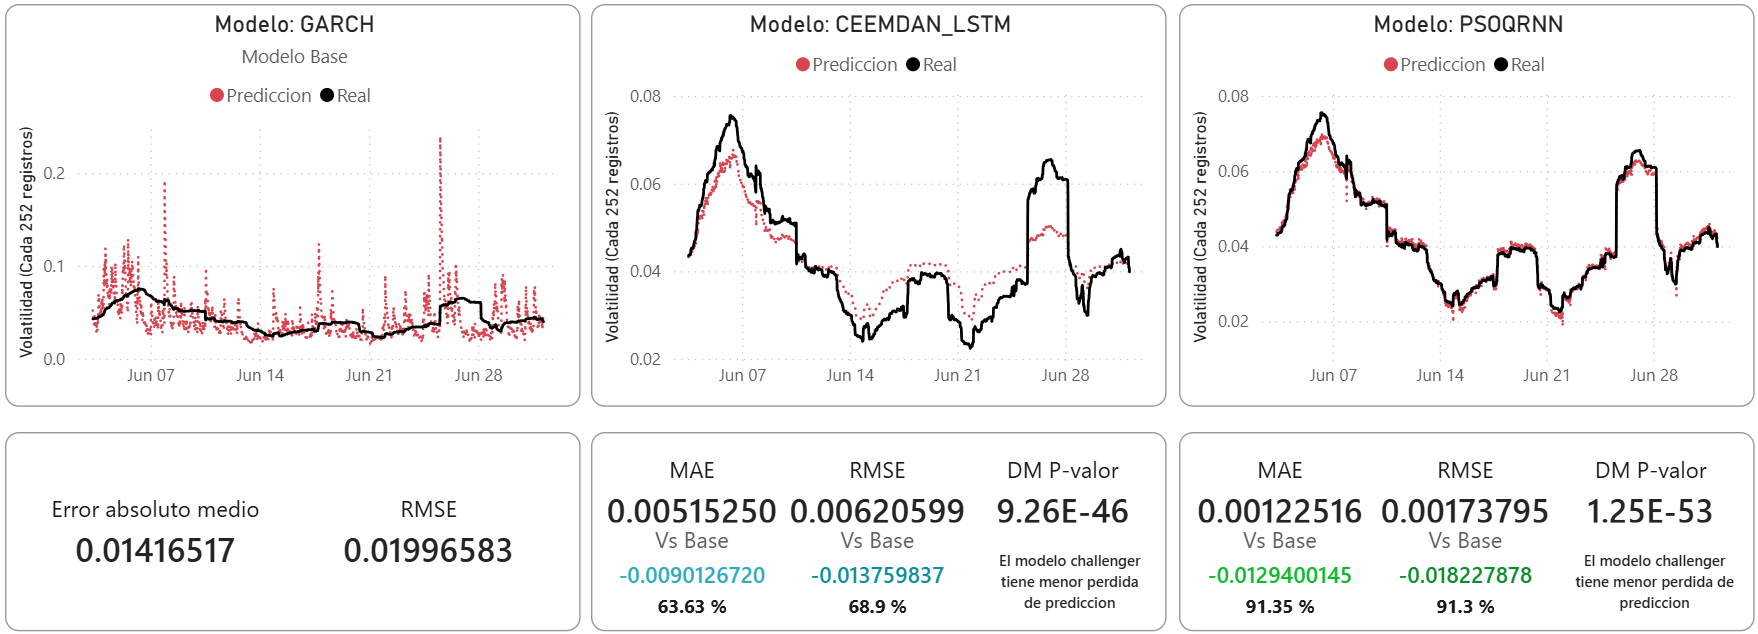
\includegraphics[width=\textwidth]{las_figuras/bitcoin.png}
    \caption{Predicción de la volatilidad del Bitcoin (BTC-USD) en el conjunto de prueba. Los modelos CEEMDAN-LSTM y PSOQRNN se comparan contra el GARCH como modelo base.}
    \label{fig:bitcoin}
\end{figure}

El Bitcoin constituye el activo con mayor número de observaciones de prueba y presenta una volatilidad intradía elevada con racimos pronunciados. Como se observa en la Figura~\ref{fig:bitcoin}, el modelo GARCH sobreestima sistemáticamente la volatilidad, produciendo predicciones muy por encima de los valores realizados. El modelo PSOQRNN logra el mejor ajuste visual y numérico: obtiene un MAE de $1{,}23 \times 10^{-3}$ y un RMSE de $1{,}74 \times 10^{-3}$, lo que representa una reducción del 91{,}3\,\% en RMSE respecto al GARCH ($p$-valor DM $= 1{,}25 \times 10^{-53}$, $p \ll 0.001$). El modelo CEEMDAN-LSTM ocupa la posición intermedia con MAE de $5{,}15 \times 10^{-3}$ y RMSE de $6{,}21 \times 10^{-3}$ (reducción del 68{,}9\,\% en RMSE, $p$-valor DM $= 9{,}26 \times 10^{-46}$), con mejoras también estadísticamente significativas frente a la línea base, aunque inferiores a las del PSOQRNN. El orden de desempeño es: PSOQRNN $>$ CEEMDAN-LSTM $>$ GARCH.

\subsection{Ethereum (ETH-USD)}

\begin{figure}[H]
    \centering
    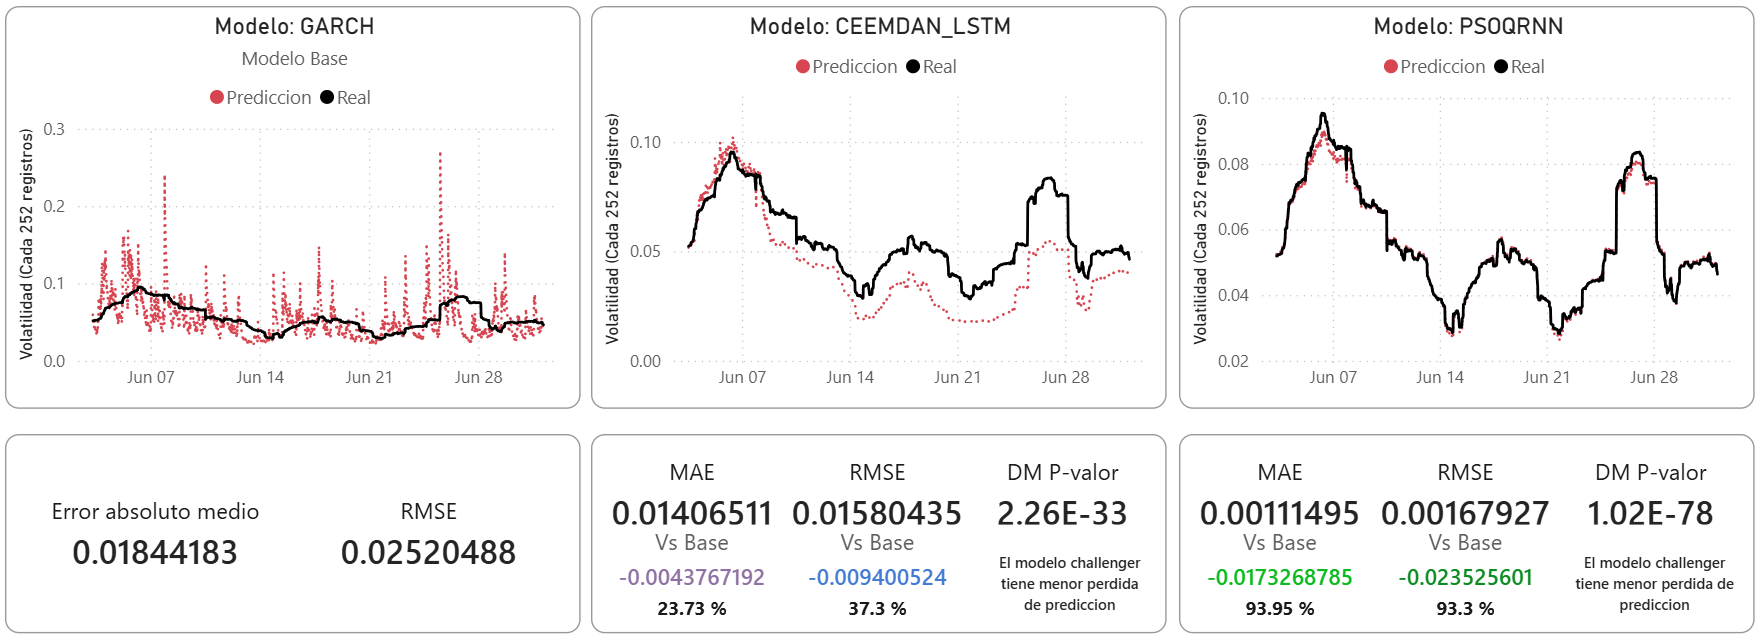
\includegraphics[width=\textwidth]{las_figuras/ethereum.png}
    \caption{Predicción de la volatilidad del Ethereum (ETH-USD) en el conjunto de prueba.}
    \label{fig:ethereum}
\end{figure}

El Ethereum presenta un perfil de volatilidad similar al Bitcoin pero con episodios de alta variabilidad más abruptos. Como se aprecia en la Figura~\ref{fig:ethereum}, el PSOQRNN mantiene la mejor capacidad de seguimiento de la serie, obteniendo un MAE de $1{,}11 \times 10^{-3}$ y un RMSE de $1{,}68 \times 10^{-3}$ (reducción del 93{,}3\,\% en RMSE respecto al GARCH, $p$-valor DM $= 1{,}02 \times 10^{-78}$). En los picos de mayor amplitud el PSOQRNN tiende a subestimar ligeramente la magnitud, lo cual se refleja en errores puntuales más elevados sin afectar significativamente las métricas globales. El CEEMDAN-LSTM también supera al GARCH con un MAE de $1{,}41 \times 10^{-2}$ y RMSE de $1{,}58 \times 10^{-2}$ (reducción del 37{,}3\,\%, $p$-valor DM $= 2{,}26 \times 10^{-33}$), aunque con menor margen que en Bitcoin. El GARCH presenta la sobreestimación sistemática observada en todos los activos. El orden de desempeño es: PSOQRNN $>$ CEEMDAN-LSTM $>$ GARCH.

\subsection{Euro/Dólar (EUR/USD)}

\begin{figure}[H]
    \centering
    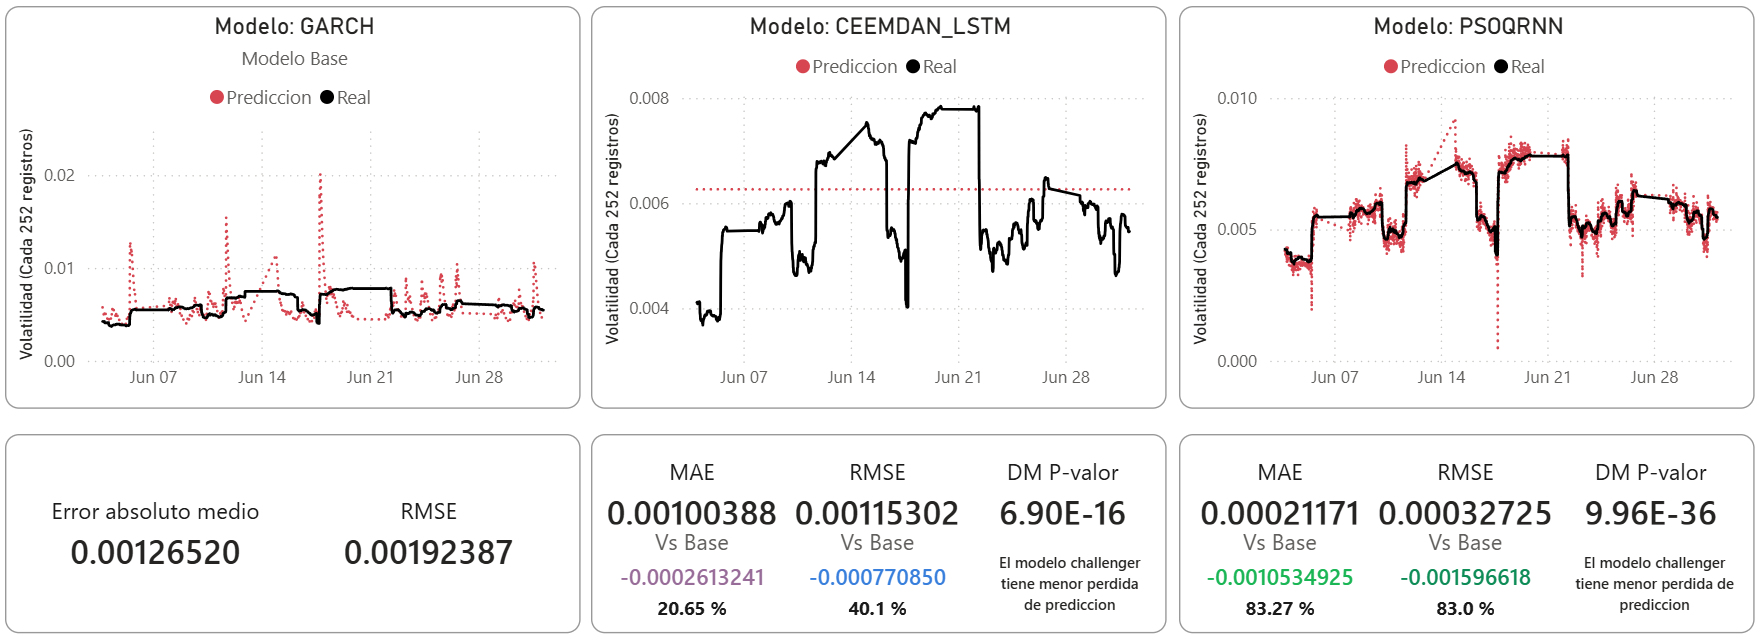
\includegraphics[width=\textwidth]{las_figuras/eurusd.png}
    \caption{Predicción de la volatilidad del par de divisas EUR/USD en el conjunto de prueba.}
    \label{fig:eurusd}
\end{figure}

El par EUR/USD corresponde al mercado de divisas, caracterizado por una volatilidad intradía generalmente más baja y con menor persistencia que las criptomonedas. A diferencia del menor margen de mejora relativa observado en ETH-USD (37\,\%), en el par EUR/USD el modelo CEEMDAN-LSTM logra capturar eficientemente la dinámica de la serie y supera al GARCH, obteniendo un MAE de $1{,}00 \times 10^{-3}$ y un RMSE de $1{,}15 \times 10^{-3}$ (reducción del 40{,}1\,\% en RMSE, $p$-valor DM $= 6{,}90 \times 10^{-16}$). El PSOQRNN vuelve a ser el modelo superior con MAE de $2{,}12 \times 10^{-4}$ y RMSE de $3{,}27 \times 10^{-4}$ (reducción del 83{,}0\,\%, $p$-valor DM $= 9{,}96 \times 10^{-36}$). El GARCH muestra el peor desempeño en este activo, con dificultades para modelar la baja persistencia de la volatilidad en divisas. El orden de desempeño es: PSOQRNN $>$ CEEMDAN-LSTM $>$ GARCH.

\subsection{Oro (GC=F)}

\begin{figure}[H]
    \centering
    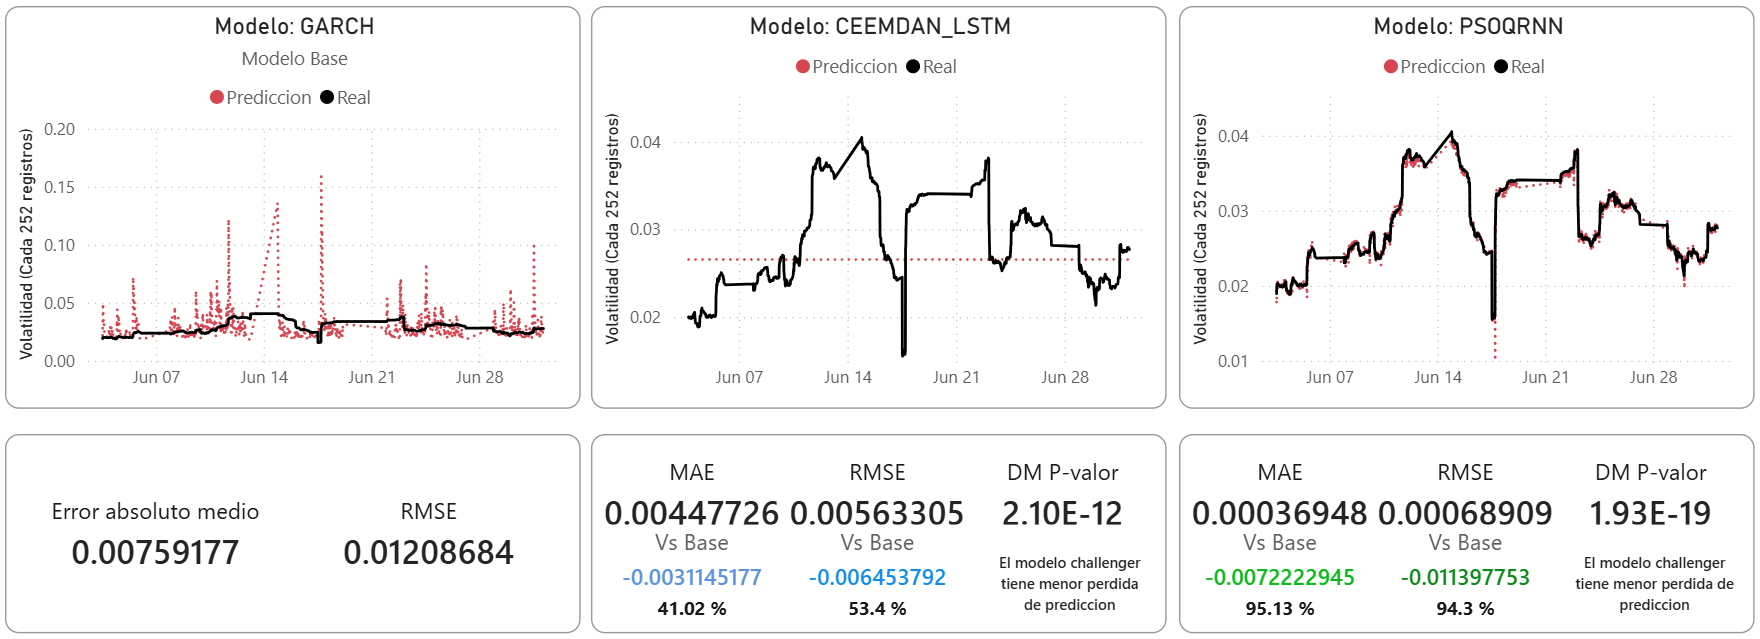
\includegraphics[width=\textwidth]{las_figuras/gold.png}
    \caption{Predicción de la volatilidad del Oro (GC=F) en el conjunto de prueba.}
    \label{fig:gold}
\end{figure}

El oro presenta una volatilidad relativamente estable con episodios de variabilidad moderada. El modelo CEEMDAN-LSTM logra en este activo identificar la dirección de los picos de volatilidad, aunque con una amplitud que no reproduce fielmente la magnitud observada, obteniendo MAE de $4{,}48 \times 10^{-3}$ y RMSE de $5{,}63 \times 10^{-3}$ (reducción del 53{,}4\,\% en RMSE, $p$-valor DM $= 2{,}10 \times 10^{-12}$). El GARCH sobreestima la variabilidad con MAE de $7{,}59 \times 10^{-3}$ y RMSE de $1{,}21 \times 10^{-2}$. El PSOQRNN obtiene la mejor precisión cuantitativa con MAE de $3{,}69 \times 10^{-4}$ y RMSE de $6{,}89 \times 10^{-4}$, lo que corresponde a una reducción del 94{,}3\,\% en RMSE respecto al GARCH ($p$-valor DM $= 1{,}93 \times 10^{-19}$, $p \ll 0.001$). El orden de desempeño es: PSOQRNN $>$ CEEMDAN-LSTM $>$ GARCH.

\subsection{S\&P\,500 (\^{}GSPC)}

\begin{figure}[H]
    \centering
    
\includegraphics[width=\textwidth]{las_figuras/sp500.png}
    \caption{Predicción de la volatilidad del índice S\&P\,500 en el conjunto de prueba.}
    \label{fig:sp500}
\end{figure}

El S\&P\,500 opera exclusivamente en días hábiles y en horario de mercado, lo que reduce su conjunto de prueba a $n = 471$ observaciones. A pesar de esta restricción, tanto el PSOQRNN como el CEEMDAN-LSTM superan ampliamente al GARCH. El CEEMDAN-LSTM obtiene MAE de $1{,}65 \times 10^{-3}$ y RMSE de $1{,}74 \times 10^{-3}$ (reducción del 91{,}0\,\% en RMSE, $p$-valor DM $= 2{,}43 \times 10^{-10}$). El PSOQRNN es el mejor modelo con MAE de $6{,}12 \times 10^{-4}$ y RMSE de $9{,}82 \times 10^{-4}$ (reducción del 94{,}9\,\%, $p$-valor DM $= 1{,}51 \times 10^{-11}$), aunque visualmente se observa que los picos de mayor amplitud no son reproducidos con la proporción exacta. El orden de desempeño es: PSOQRNN $>$ CEEMDAN-LSTM $>$ GARCH.

\subsection{NASDAQ (\^{}IXIC)}

\begin{figure}[H]
    \centering
    
\includegraphics[width=\textwidth]{las_figuras/nasdaq.png}
    \caption{Predicción de la volatilidad del índice NASDAQ en el conjunto de prueba.}
    \label{fig:nasdaq}
\end{figure}

El NASDAQ comparte con el S\&P\,500 las mismas restricciones de operación como índice bursátil ($n = 476$ observaciones en el conjunto de prueba). El CEEMDAN-LSTM obtiene MAE de $1{,}00 \times 10^{-3}$ y RMSE de $1{,}23 \times 10^{-3}$ (reducción del 95{,}3\,\% en RMSE respecto al GARCH, $p$-valor DM $= 3{,}15 \times 10^{-9}$), logrando su segunda mejor reducción relativa en todo el estudio. El PSOQRNN mantiene el primer lugar con MAE de $6{,}99 \times 10^{-4}$ y RMSE de $9{,}95 \times 10^{-4}$ (reducción del 96{,}2\,\%, $p$-valor DM $= 1{,}09 \times 10^{-9}$). El GARCH, con RMSE de $2{,}59 \times 10^{-2}$, muestra una sobreestimación especialmente pronunciada en este activo. El orden de desempeño es: PSOQRNN $>$ CEEMDAN-LSTM $>$ GARCH.

\subsection{Resumen comparativo}

La Tabla~\ref{tab:resumen_metricas} consolida los resultados de MAE y RMSE de los tres modelos para todos los activos evaluados, junto con los $p$-valores del test de Diebold--Mariano de cada modelo \textit{challenger} respecto al GARCH. El resultado más destacado es la consistencia del PSOQRNN como modelo superior en los seis activos, con reducciones de RMSE respecto al GARCH que oscilan entre el 83\,\% (EUR/USD) y el 96\,\% (NASDAQ). El CEEMDAN-LSTM también supera al GARCH en todos los activos con diferencias estadísticamente significativas, con reducciones de RMSE entre el 37\,\% (ETH-USD) y el 95\,\% (NASDAQ). El GARCH muestra sistemáticamente la mayor sobreestimación de la volatilidad en todos los activos evaluados.

\begin{table}[H]
\centering
\caption{Comparación de métricas de error (MAE y RMSE) por modelo y activo. Los mejores valores por activo se indican en negrita. La columna DM $p$-val reporta el $p$-valor del test de Diebold--Mariano del modelo \textit{challenger} vs. GARCH ($H_0$: igual pérdida de predicción). Todos los $p$-valores $\ll 0.001$.}
\label{tab:resumen_metricas}
\resizebox{\textwidth}{!}{%
\begin{tabular}{llrr|rrr|rrr}
\hline
\multirow{2}{*}{\textbf{Activo}} & \multirow{2}{*}{\textbf{Clase}} &
  \multicolumn{2}{c|}{\textbf{GARCH}} &
  \multicolumn{3}{c|}{\textbf{CEEMDAN-LSTM}} &
  \multicolumn{3}{c}{\textbf{PSOQRNN}} \\
\cline{3-10}
 & & MAE & RMSE & MAE & RMSE & DM $p$-val & MAE & RMSE & DM $p$-val \\
\hline
BTC-USD  & Cripto     & $1.42\times10^{-2}$ & $2.00\times10^{-2}$ & $5.15\times10^{-3}$ & $6.21\times10^{-3}$ & $9.3\times10^{-46}$ & $\mathbf{1.23\times10^{-3}}$ & $\mathbf{1.74\times10^{-3}}$ & $1.2\times10^{-53}$ \\
ETH-USD  & Cripto     & $1.84\times10^{-2}$ & $2.52\times10^{-2}$ & $1.41\times10^{-2}$ & $1.58\times10^{-2}$ & $2.3\times10^{-33}$ & $\mathbf{1.11\times10^{-3}}$ & $\mathbf{1.68\times10^{-3}}$ & $1.0\times10^{-78}$ \\
EUR/USD  & Divisa     & $1.27\times10^{-3}$ & $1.92\times10^{-3}$ & $1.00\times10^{-3}$ & $1.15\times10^{-3}$ & $6.9\times10^{-16}$ & $\mathbf{2.12\times10^{-4}}$ & $\mathbf{3.27\times10^{-4}}$ & $1.0\times10^{-35}$ \\
GC=F     & Mat. prima & $7.59\times10^{-3}$ & $1.21\times10^{-2}$ & $4.48\times10^{-3}$ & $5.63\times10^{-3}$ & $2.1\times10^{-12}$ & $\mathbf{3.69\times10^{-4}}$ & $\mathbf{6.89\times10^{-4}}$ & $1.9\times10^{-19}$ \\
\^{}GSPC  & Índice     & $1.36\times10^{-2}$ & $1.93\times10^{-2}$ & $1.65\times10^{-3}$ & $1.74\times10^{-3}$ & $2.4\times10^{-10}$ & $\mathbf{6.12\times10^{-4}}$ & $\mathbf{9.82\times10^{-4}}$ & $1.5\times10^{-11}$ \\
\^{}IXIC  & Índice     & $1.77\times10^{-2}$ & $2.59\times10^{-2}$ & $1.00\times10^{-3}$ & $1.23\times10^{-3}$ & $3.2\times10^{-9}$  & $\mathbf{6.99\times10^{-4}}$ & $\mathbf{9.95\times10^{-4}}$ & $1.1\times10^{-9}$  \\
\hline
\end{tabular}%
}
\end{table}

\section{Conclusiones y recomendaciones}

Este trabajo comparó tres metodologías de modelamiento de volatilidad en series financieras intradía —GARCH, CEEMDAN-LSTM y PSOQRNN— sobre seis activos de clases diferenciadas: criptomonedas (Bitcoin y Ethereum), divisas (EUR/USD), materias primas (Oro) e índices bursátiles (S\&P\,500 y NASDAQ). Los resultados permiten extraer las siguientes conclusiones.

\textbf{Superioridad consistente del PSOQRNN.} El modelo PSOQRNN obtuvo el mejor desempeño en los seis activos evaluados, con reducciones de RMSE respecto al GARCH que oscilan entre el 83\,\% (EUR/USD) y el 96\,\% (NASDAQ). En todos los casos, el test de Diebold--Mariano confirmó que esta diferencia es estadísticamente significativa ($p \ll 0.001$). La capacidad del PSOQRNN para estimar el cuantil condicional de la volatilidad, combinada con la robustez del PSO para escapar de mínimos locales, se traduce en un ajuste consistentemente superior frente al enfoque paramétrico clásico.

\textbf{CEEMDAN-LSTM como alternativa sólida.} El modelo CEEMDAN-LSTM supera al GARCH en todos los activos evaluados con diferencias estadísticamente significativas, logrando reducciones de RMSE entre el 37\,\% (ETH-USD) y el 95\,\% (NASDAQ). El mecanismo de descomposición modal adaptativa permite separar los componentes de frecuencia de la serie antes del entrenamiento, lo que reduce el efecto del ruido y mejora la capacidad predictiva de la red LSTM. No obstante, su ventaja relativa frente al PSOQRNN es menor, especialmente en activos de alta volatilidad como las criptomonedas.

\textbf{Limitaciones del modelo GARCH.} El GARCH mostró sistemáticamente la mayor sobreestimación de la volatilidad en todos los activos. Este comportamiento es consistente con las limitaciones conocidas de los modelos paramétricos para series intradía: los supuestos de linealidad, la dependencia de la especificación de la distribución de los errores y la incapacidad de capturar cambios estructurales abruptos limitan su desempeño en entornos de alta frecuencia y elevada variabilidad. Sin embargo, el GARCH sigue siendo valioso como referencia de desempeño mínimo esperado y como herramienta para la selección del modelo de media mediante AIC.

\textbf{Eficiencia computacional.} El costo de entrenamiento de las redes neuronales con GPU es comparable al de la estimación del GARCH para series de longitud similar. Sin embargo, en la fase de inferencia, las redes son considerablemente más rápidas y no requieren reestimación del modelo al incorporar nuevas observaciones, lo que las hace más adecuadas para aplicaciones de pronóstico en tiempo real.

\textbf{Limitaciones del estudio.} El presente trabajo presenta las siguientes limitaciones que deben considerarse al interpretar los resultados: (i) los hiperparámetros de los modelos de redes neuronales se fijaron de forma global para todos los activos, sin optimización específica por clase de instrumento; (ii) la cobertura temporal está acotada al período febrero--julio de 2026, lo que limita la generalización de los resultados a otros regímenes de mercado; (iii) los índices bursátiles cuentan con un conjunto de prueba significativamente más reducido que los activos de operación continua.

\textbf{Recomendaciones para trabajo futuro.} Con base en los hallazgos del estudio se proponen las siguientes líneas de investigación: (i) realizar una optimización de hiperparámetros específica por activo o clase de instrumento, con especial énfasis en el número de neuronas ocultas del QRNN y los parámetros del PSO; (ii) extender la ventana de datos mediante la acumulación progresiva del módulo de obtención, lo que permitiría una evaluación más robusta en distintos regímenes de volatilidad; (iii) explorar esquemas de reentrenamiento periódico de los modelos de redes neuronales para capturar derivas estructurales en la dinámica de la volatilidad; (iv) evaluar el desempeño de enfoques de ensamble que combinen las predicciones de los tres modelos, aprovechando sus fortalezas complementarias.


\newpage
\bibliographystyle{apalike}
\bibliography{mi_bibliografia}

\end{document}
